\documentclass[a4paper,english]{report}
\usepackage[utf8]{inputenc}
\usepackage[english]{babel}
\usepackage{frontpage/uiomasterfp}
\usepackage{hyperref}
\usepackage{biblatex}
\usepackage{csquotes}
\usepackage{caption}
\usepackage{subfig}
\usepackage{amsthm}
\usepackage{tikz-qtree}
\usepackage{amsmath}


\usepackage{graphicx}
\usepackage{amsmath}
\usepackage{tikz}
\usepackage[a4paper, total={}]{geometry}
\usepackage{tcolorbox}
\setlength{\headsep}{5pt}
\setlength{\parskip}{1em}
\usepackage{listings}
\usepackage{extarrows}
\usepackage{bold-extra}

\usepackage{algorithm2e}


\definecolor{pblue}{rgb}{0.2,0.2,0.7}
\definecolor{pgreen}{rgb}{0,0.5,0}
\definecolor{pred}{rgb}{0.7,0.2,0.2}
\definecolor{pgrey}{rgb}{0.46,0.45,0.48}

\lstset{
  language=Java,
  showstringspaces=false,
  columns=flexible,
  basicstyle={\small\ttfamily},
  numbers=none,
  numberstyle=\tiny\color{gray},
  keywordstyle=\color{blue},
  commentstyle=\color{pgreen},
  stringstyle=\color{mauve},
  breaklines=true,
  breakatwhitespace=true,
  tabsize=3
}



\addbibresource{refs.bib}

\newtheorem{definition}{Definition}
\newtheorem{theorem}{Theorem}

\def\addsquare#1{\tikz\node[draw]{#1};}
\def\addcircle#1{\tikz\node[draw,circle]{#1};}

\title{CC-LSP: Language and IDE agnostic code clone detection}
\subtitle{Incremental code clone detection for text editors}


\author{Jakob Konrad Hansen}
\begin{document}

\SetKwFunction{max}{max}
\SetKwFunction{min}{min}

\SetKwProg{algo}{Algorithm}{}{}
\SetKwFunction{access}{access}
\SetKwFunction{isLeaf}{isLeaf}
\SetKwFunction{bwt}{BWT}


\SetKwFunction{ISA}{ISA}
\SetKwFunction{LCP}{LCP}



% \duoforside[dept={Department of Informatics},
% program={Informatics: Programming and System Architecture},
% long]
\uiomasterfp[color=blue]


\chapter*{Abstract}

Duplicated code, code which is more or less copied to different locations in a code base
is present in almost all software today. This can especially affect the maintainability
and extensibility of the software. Algorithms and tools which facilitates detection and
management of duplicated codes is therefore an important research field. Incremental
detection algorithms, algorithms which do not need to run the entire analysis from scratch
for consecutive revisions of the code base, is especially interesting for use cases such
as when running the detection tool in an IDE. In this thesis we present CCDetect-LSP, a
duplicate code detection tool which targets the IDE scenario and implements a novel
incremental clone detection algorithm, which aims to be faster than rerunning the analysis
from scratch.


\tableofcontents

\chapter{Introduction}

Refactoring is the process of restructuring source code in order to improve the internal
behavior of the code, without changing the external behavior~\cite[9]{fowlerrefactoring}.
Refactoring source code is often performed in order to eliminate instances of bad code
quality, otherwise known as code smells.

A study conducted by Diego Cedrim et al. has shown that while programmers tend to refactor
smelly code, they are rarely successful at eliminating the smells they are
targeting~\cite{Rohit_Gheyi_Impact}. Most refactorings performed were either
``smell-neutral'', meaning that the targeted code smell is not eliminated, or ``stinky'',
meaning that the refactoring introduced more code smells than they eliminated. Automated
tools that help programmers make better refactorings and perform code analysis could be a
solution to this problem. 

Duplicate code, often called code clones, is code which is more or less copied to
different locations in a code base. Code clones occur in practically every large software
project, and code clone analysis has therefore become a highly active field of research in
the last decade. Many tools and algorithms have been developed to detect, manage and
refactor code clones~\cite[6]{Inoue_introduction_to_cc}. Code clone detection in large
software can be a time-consuming process. A consequence of this is that few existing tools
are highly integrated into the workflow of software developers and are not designed to be
run on a code base every time the code base changes. This thesis will therefore focus
on efficient code clone detection and presents a novel algorithm and tool for detecting
code clones in a real-time programming environment.

\section{Motivation and problem statement}

Many tools and algorithms exist for code clone detection. However, few of these have the
capability of efficiently detecting clones in a real-time programming environment. A
problem with existing algorithms is that most of them need to rerun the entire analysis
whenever a change to a file happens. Incremental algorithms that do not recompute all
clones from scratch are therefore interesting for use-cases such as while programming in
integrated development environments (IDEs) and for analyzing different revisions of the
same source code, but this type of algorithm has not been thoroughly explored for code
clone analysis.

Our proposed solution and tool addresses this issue by introducing a new algorithm that is
capable of detecting and updating existing code clones as source code changes, which aims
to be faster than redoing the analysis from scratch. CCDetect-LSP, the tool which
implements this algorithm, is also programming language- and IDE agnostic, allowing
programmers to seamlessly incorporate the detection of duplicated code into their existing
development environment.

\section{Our contribution}

CCDetect-LSP provides exact code clone detection capabilities in a real-time IDE
environment. The tool allows the user to list and interact with all the clones in the code
base, jump between matching clones, and get fast feedback while editing code in order to
determine which clones are introduced or eliminated.

Existing incremental clone detection tools either do not fit into an IDE scenario, are
limited in terms of what clones they display, or have not been shown to scale well in
terms of processing time or memory usage for larger codebases. Therefore, this thesis will
focus on the following areas.

\textbf{Incremental clone detection:} The main focus of this thesis is making the tool
efficient in terms of incrementally updating the analysis whenever edits are performed in
the IDE. Most clone detection algorithms either only list clones of a specific code
snippet, or calculates clones from scratch in a manner which is too slow for an IDE
scenario. Our algorithm is based on a novel application and extension of dynamic suffix
arrays for clone detection, which can be efficiently updated and find clones. While suffix
arrays have been used for clone detection before~\cite{SHINOBI}, we are not aware of any
other attempts to use suffix arrays in an incremental setting. With this algorithm,
CCDetect-LSP can display all clones in the entire code base at once, and efficiently
update the displayed clones whenever a file is edited.

\textbf{IDE and language agnostic clone detection:} CCDetect-LSP gives programmers the
ability to view clones in their IDE. Utilizing features of the language server protocol
(LSP) such as diagnostics and code-actions~\cite{lsp}, the tool provides clone analysis to
any editor which implements the LSP protocol. As far as we are aware there are no other
clone detection tools which utilizes LSP to provide clone analysis. In addition, the tool
is also language agnostic in the sense that it only needs a grammar for the parser
generator Tree-sitter, for it to be analyzed~\cite{treesitter}. 

\section{Structure}

Chapter 2 provides background on code clone analysis, existing tools and preliminary
algorithms and data structures used in the implementation. Chapter 3-5 describes the
implementation of CCDetect-LSP and the algorithms used for initial and incremental clone
detection. In chapter 6, the tool is evaluated based on multiple criteria, and compared to
other existing solutions. Chapter 7 discusses the results of the evaluation. Chapter 8
lists related and future work, and concludes the thesis.

\chapter{Background}


\section{Software quality and duplicated code}

Software quality is hard to define. The term ``quality'' is ambiguous and is in the case
of software quality, multidimensional. Quality in itself has been defined as ``conformance
to requirements''~\cite[8]{crosby1980quality}. In software, a simple measure of
``conformance to requirements'' is correctness, and a lack of bugs. However, software
quality is often measured in other metrics, including metrics which are not directly
related to functionality~\cite[29]{MetricsAndModelsInSoftwareQuality}. Whenever duplicated
code needs to changed, it will require changes in multiple locations, meaning that metrics
such as maintainability, analyzability and changeability are negatively affected.

These metrics are affected negatively by duplicated code. Multiple studies have shown that
software projects typically contains $10-15\%$ duplicated code~\cite{CloningByAccident}.
Therefore, research into tools and techniques which can assist in reducing duplicated code
will be of benefit to almost all software.

Duplicated code can lead to a plethora of anti-patterns. Anti-patterns are bad design
decisions for software which can lead to technical debt. Technical debt occurs when
developers make technical compromises that are expedient in the short term, but increases
complexity in the long-term~\cite[111]{TechnicalDebt}. An example of this, in the context
of duplicated code, is the ``Shotgun-Surgery''~\cite[66]{fowlerrefactoring} anti-pattern.
This anti-pattern occurs when a developer wants to implement a change, but needs to change
code at multiple locations for the change to take effect. This is a typical situation
which slows down development and reduces maintainability when the amount of duplicated
code increases in a software project.

\section{Code clones}

Duplicated code is often described as ``code clones'', a pair of code snippets which are
duplicated are considered clones of each other.

\begin{definition}[Code snippet]
	A code snippet is a piece of contiguous source code in a larger software system.
\end{definition}

\begin{definition}[Code clone]
	A code clone is a code snippet which is equal to or similar to another code snippet. The two
	code snippets are both code clones, and together they form a code clone pair.
	Similarity is determined by some metric such as number of equal lines of code.
\end{definition}

\begin{definition}[Clone class]
	A clone class is a set of code snippets where all snippets are considered clones of each
	other.
\end{definition}


The clone relation is a relation between code snippets which defines pairs of clones.
The clone relation is reflexive and symmetric, but not necessarily transitive. The transitive
property depends on the threshold for similarity when identifying code clones. Given

$$a \xleftrightarrow{clone} b \xleftrightarrow{clone} c$$


where $a,b,c$ are code snippets and $\xleftrightarrow{clone}$ gives the clone relation.
$a$ and $c$ are both clones of $b$, but not necessarily similar enough to be clones of
each other, depending on the threshold for similarity. If the threshold for similarity is
defined such that only equal clones are considered clones, the relation becomes
transitive, and equivalence classes form clone classes.

Code clones are generally classified into four types~\cite{Inoue_introduction_to_cc}. The
types classify code snippets as code clones with an increasing amount of leniency.
Therefore, Type-1 code clones are very similar, while Type-4 clones are not necessarily
syntactically similar at all. When defining types, it is the syntactic and structural
differences which is compared, not functionality. The set of code clones classified by a
code clone type is also a subset of the next type, meaning all Type-1 clones are also
Type-2 clones, but not vice versa.

The code clone types are defined as follows:

\textbf{Type-1} clones are syntactically identical. The only differences allowed are elements
without meaning, like comments and white-space. Example:

\Todo{Redo these}
\begin{tcolorbox}
	\begin{center}
		\begin{tabular}{c | c}
            \begin{lstlisting}
for (int i = 0; i < 10;   i++) {

    print(i);
}
        \end{lstlisting} &
			\begin{lstlisting}

for (int i = 0; i < 10; i++) {
    // A comment

    print(i);
}
        \end{lstlisting}
		\end{tabular}
	\end{center}
\end{tcolorbox}


\textbf{Type-2} clones are structurally identical. Possible differences include
identifiers, literals and types. Type-2 clones are not much harder to detect than type-1
clones, since consistently renaming identifiers, literals and types allow a type-1
detection algorithm to find type-2 clones~\cite{Zibran_real_time_search}. This type of
clone is relevant to consider in refactoring scenarios when merging code clones. This is
because type-2 clones can be relatively simple to parameterize in order to hide the
differences in the merged code, and allows the original locations of clones to be replaced
with a call to the merged code, with different parameters. Example:

\begin{center}
	\begin{tcolorbox}
		\begin{tabular}{c | c}
			\begin{lstlisting}
for (int i = 0; i < 10; i++) {
    print(i);
}
    \end{lstlisting} &
	\begin{lstlisting}
for (int (*\textbf j*) = (*\textbf 1*); (*\textbf j*) < 10; (*\textbf j++*)) {
    print((*\textbf j*));
}
    \end{lstlisting}
		\end{tabular}
	\end{tcolorbox}
\end{center}

\textbf{Type-3} clones are required to be structurally similar, but not equal. Differences
include statements that are added, removed or modified. This clone type relies on a
threshold $\theta$ which determines how structurally different snippets can be in order to
be considered Type-3 clones~\cite{Inoue_introduction_to_cc}. The granularity for this
difference could be based on differing tokens, lines, etc. Detecting this type of clone is
hard. Example:

\begin{tcolorbox}
	\begin{center}
		\begin{tabular}{c | c}
			\begin{lstlisting}
// Clone 1
for (int i = 0; i < 10; i++) {
    print(i);
}
\end{lstlisting} &
			\begin{lstlisting}
// Clone 2
for (int i = 0; i < 10; i++) {
    print(i);
    (*\textbf{int x = 10;}*)
}
\end{lstlisting}
		\end{tabular}
	\end{center}
\end{tcolorbox}




In this example there is a one line difference between the two snippets, so if $\theta
	\geq
	1$, the two snippets would be considered Type-3 clones.

\textbf{Type-4} clones have no requirement for syntactical or structural similarity, but
are generally only relevant to detect when they have similar functionality. Detecting this
type of clone is very challenging, but attempts have been made using program dependency
graphs~\cite{SeedType4Detection}. The following example shows two code snippets which have
no clear syntactic or structural similarity, but is functionally equal:

\begin{tcolorbox}
	\begin{center}
		\begin{tabular}{c | c}
			\begin{lstlisting}
print((n*(n-1))/2)
\end{lstlisting} &
			\begin{lstlisting}
int sum = 0;
for (int i = 0; i < n; i++) {
    for (int j = i+1; j < n; j++) {
        sum++;
    }
}
print(sum);
\end{lstlisting}
		\end{tabular}
	\end{center}
\end{tcolorbox}


Type-1 clones are often referred to as ``exact'' clones, while Type-2 and Type-3 clones
are referred to as ``near-miss'' clones~\cite[1]{Zibran_real_time_search}.

\section{Code clone detection process and techniques}

\textbf{The Code clone detection process} is generally split into (but is not limited to)
a sequence of steps to identify clones~\cite{Inoue_introduction_to_cc}. This
process is often a pipeline of input-processing steps before finally comparing fragments
against each other and filtering. The steps are generally as follows:

\begin{enumerate}
	\item \textbf{Pre-processing}: Filter uninteresting code that we do not want to
	      check for clones, for example generated code. Then partition code into a set of
	      fragments, depending on granularity such as methods, files or lines.
	\item \textbf{Transformation}: Transform fragments into an intermediate
	      representation, with a source-map back to the original code. An algorithm
          could potentially do multiple transformation before arriving at the wanted
          representation
	      \begin{enumerate}
		      \item Extraction: Transform source code into the input for the comparison
		            algorithm. Can be tokens, AST, dependency graphs, suffix tree, etc.
		      \item Normalization: Optional step which removes superficial differences such as
		            comments, whitespace and identifier names. Often useful for identifying type-2
		            clones.
	      \end{enumerate}
	\item \textbf{Match detection}: Perform comparisons which outputs a set of
	      candidate clone pairs.
	\item \textbf{Source-mapping / Formatting}: Convert candidate clone pairs from the transformed
	      code back to clone pairs in the original source code.
	\item \textbf{Post-processing / Filtering}: Ranking and filtering manually or with
	      automated heuristics
	\item \textbf{Aggregation}: Optionally aggregating sets of clone pairs into clone sets
\end{enumerate}

\paragraph{Matching techniques} are techniques which can be applied to source-code to
detect clone-pairs. Most matching technique will also require specific pre-processing to be
done in the earlier steps, for example building an AST. Some of the most explored
techniques are as follows~\cite{ComparisonAndEvaluationOfTechniques}:

\paragraph{Text-based} approaches do little processing of the source code before
comparing. Simple techniques such as fingerprinting or incremental hashing have been used
in this approach. Dot-plots have also been used in newer text-based approaches, placing
the hashes of fragments in a dot plot for use in comparisons.

\paragraph{Token-based} approaches transform source code into a stream of tokens, similar
to lexical scanning in compilers. The token stream is then scanned for duplicated
subsequences of tokens. Since token streams can easily filter out superficial differences
such as whitespace, indentation and comments, this approach is more robust to such
differences. Concrete names of identifiers and values can be abstracted away when
comparing the token-stream, therefore Type-2 clones can easily be identified. Type-3
clones can also be identified by comparing the fragments tokens and keeping clone pairs
with a lexical difference lower than a given threshold. This can be solved with dynamic
programming~\cite{BakerSparseDynamicProgramming}. A common approach to detect clones using
token-streams is with a suffix-tree~\cite{Zibran_real_time_search}. A suffix-tree can solve
the \textit{Find all maximal repeats} problem efficiently, which in essence is the same
problem as finding clone pairs. A similar algorithm can also be performed using a suffix-array
instead, which requires less memory. This type of code clone detection is very fast
compared to more intricate types of matching techniques.

\paragraph{Syntactic} approaches transform source code into either concrete syntax trees
or abstract syntax trees and find clones using either tree matching algorithms or
structural metrics. For tree matching, the common approach is to find similar subtrees,
which are then deemed as clone pairs. One way of finding similar subtrees is to compare
subtrees with a tolerant tree matching algorithm for detecting type-3
clones~\cite{ASTCloneDetection}. Variable names, literal values and types may be
abstracted to find type-2 clones more easily. Metrics-based techniques gather metrics for
code fragments in the tree and uses the metrics to determine if the fragments are clones
or not. One way is to use fingerprint functions where the fingerprint includes certain
metrics, and compare the fingerprints of all fragments to find clones~\cite{Deckard}.

\paragraph{Hybrid} approaches combine multiple approaches in order to improve detection.
For example Zibran et al. developed a hybrid algorithm combining both token-based suffix
trees for Type-1 and Type-2 clone detection, with a k-difference dynamic programming
algorithm for Type-3 clone detection~\cite{Zibran_real_time_search}.


\section{Incremental clone detection}

Incremental clone detection involves avoiding recalculation of already calculated results
when performing code clone detection. Since most code of a codebase will not change
between revisions, a lot of processing can be avoided. However, this is not a simple
problem, since changes in a single location can affect clone detection results across the
entire codebase.

In order to incrementally detect code clones, an algorithm is run which calculates the
initial clones, and for successive revisions of the source code, this list is
incrementally updated, more efficiently than the initial run. Different algorithms will
also maintain different data structures to support detecting new clones faster in
successive revisions.

Göde and Koschke proposed the first incremental clone detection
algorithm~\cite{GodeIncrementalCloneDetection}. The algorithm employs a generalized suffix
tree in which the amount of work of updating is only dependent on the size of the edited
code. This approach requires a substantial amount of memory, and is therefore limited in
scalability.

Nguyen et al.~\cite{LocalitySensitiveHashingIncremental} showed that an AST-based approach
utilizing ``Locality-Sensitive Hashing'' can detect clones incrementally with high
precision, and showed that incremental updates could be done in real-time ($< 1$ second)
for source code with a size of 300 KLOC.

Hummel et al.~\cite{IndexBasedIncrementalCloneDetection} later introduced the first incremental,
scalable and distributed clone detection technique for Type-1 and Type-2 clones. This
approach utilizes a custom ``clone index'' data structure which can be updated
efficiently. The implementation of this data structure is similar to that of an inverted
index. This technique uses distributed computing to speed up its detection process.

More recently, Ragkhitwetsagul and Krinke~\cite{SiameseScalableAndIncrementalClone}
presented the tool ``Siamese'', which uses a novel approach of having multiple
intermediate representations of source code to detect a high number of clones with support
for incremental detection. The tool can detect up to Type-3 clones, but will only return
clones based on ``queries'' given to it by the user. Queries are either files or methods
in source-code, which are then checked for existing code clone.



\section{Code clone IDE tooling}


Developers are not always aware of the creation of clones in their code. \emph{Clone aware
development} means including clone management as a part of the software development
process. Clone aware development therefore requires programmers to be aware of and be able
to identify code clones while programming. Since large software projects can contain a lot
of duplication, it can be hard to keep track of and manage clones. Tools which help
developers locate and deal with clones can be a solution to this. However, Mathias Rieger
et al. claims that a problem with many detection tools is that the tools ``report large
amounts data that must be treated with little tool
support''~\cite[1]{InsightsSystemWideDuplication}. Detecting and eliminating clones early
in their lifecycle with IDE integrated tools could be a solution to the problem of dealing
with too many clones.

There are multiple existing clone detection tools, and the following section will go over
tools that are integrated into an IDE and offer services to the programmer while developing. Some
of these tools will 

The IDE-based tools which exist can be categorized as
follows~\cite[8]{Udding_Towards_Convenient_Management}:

\begin{itemize}
	\item\textit{Copy-paste-clones:} This category of tools deals only with code snippets which are
	copy-pasted from another location in code. These tools therefore only track clones which
	are created when copy-pasting, and does not use any other detection techniques. Therefore,
	this type of tool is not suitable for detecting clones which are made accidentally, since
	developers are aware that they are creating clones when pasting already existing code
	snippets.

	\item\textit{Clone detection and visualization tools:} This category of tools has more
	sophisticated clone detection capabilities and will detect code clones which occur
	accidentally.

	\item\textit{Versatile clone management:} This category of tools covers tools which provide more
	services than the above. Services like refactoring and simultaneous editing of clones fall
	under this category.
\end{itemize}

The following tools have been developed as IDE tools to allow for clone-aware development:

\begin{itemize}

	\item Minhaz et al. introduced a hybrid technique for performing real-time focused
	      searches, i.e. searching for code clones of a selected code snippet. This
	      technique can also detect Type-3 clones~\cite{Zibran_real_time_search}. It was
	      later used in the tool
	      \textit{SimEclipse}~\cite{Udding_Towards_Convenient_Management} which is a plugin
	      for the Eclipse editor. Since this tool can only detect clones of a code snippet
	      which the developer actively selects, this tool is not well suited for finding
	      accidental clones and tracking clones in areas.

    \item Another tool, SHINOBI, which is a plugin for the Visual Studio editor, can
        detect code clones in real-time without the need of the developer to select a code
        snippet, but the clones being displayed seem to only be clones of the source-code
        which is currently being edited. It can detect Type-1 and Type-2 code clones and
        uses a token-based suffix array approach to detect clones. The paper does not
        describe how the suffix array is updated, but as the paper was released before the
        first paper describing dynamic suffix arrays~\cite{DynamicExtendedSuffixArrays},
        one can assume that the suffix array is not dynamically updated.~\cite{SHINOBI}.

	\item The modern IDE IntelliJ has a built-in duplication detection and refactoring
	      service, it is able to detect Type-1 and (some) type-2 code clones at a method
	      granularity and refactors by replacing one of the clones with a method call to the
	      other.

\end{itemize}

\section{The Language Server Protocol}

Static analysis tools that integrate with IDEs are usually tightly coupled to a specific
IDE and its APIs, like parsing and refactoring support. This makes it difficult to utilize
a tool in another IDE, since the API's the tool utilizes is no longer available. In order
to make IDE-based static analysis tools more widely available, it is useful if such tools
could be made IDE agnostic. The Language Server Protocol (LSP) is a protocol which
attempts to solve this problem~\cite{lsp}.

LSP is a protocol which specifies interaction between a client (IDE) and server in order
to provide language tooling for the client. The goal of the protocol is to avoid multiple
implementations of the same language tools for every IDE and every language, allowing for
editor agnostic tooling. Servers which implement LSP will be able to offer IDEs
code-completion, error-messages, go-to-definition and more. LSP also specifies generic
code-actions and commands, which the LSP server provides to the client in order to perform
custom actions defined by the server.

Figure \ref{fig:lspcommunication} shows a sample interaction between client and server
using LSP. The client sends requests to a server in the form of JSON-RPC messages, and the
server sends a corresponding response, also in the form of JSON-RPC messages.

\begin{figure}[t]
	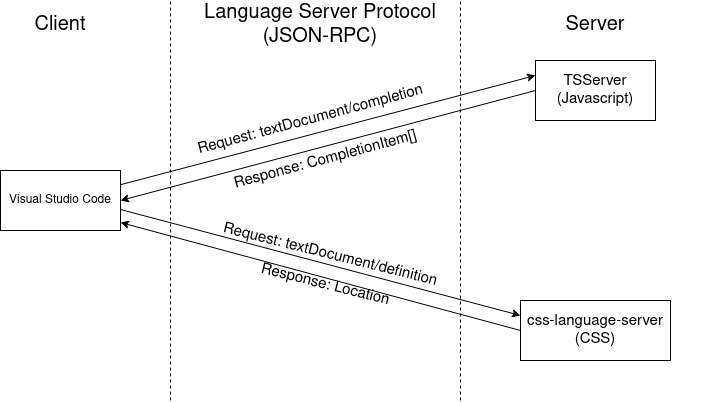
\includegraphics[width=\textwidth]{images/lspcommunication.png}
	\caption{Example client-server interaction using LSP}
	\label{fig:lspcommunication}
\end{figure}

\section{Preliminary algorithms and data structures}
\label{prelimalgos}

The following algorithms and data structures will be useful insight in following chapters to
define the detection algorithm

\subsubsection{Incremental-parsing}

While writing code, programmers usually only edit small regions of code at a time. One
``edit'' will therefore only affect small parts of the internal representations of the
code which most tools use to perform analysis. Reusing parts of this representation would
therefore be faster and allow programming tools to scale better. 

In our detection algorithm we will need to be able to parse our source code into an AST
representation in order to select specific syntactic regions and extract the tokens.
Therefore, we need a parsing algorithm, and when source code is edited we need an
incremental parsing algorithm to more efficiently parse the source code when only a
small region has been changed.

Incremental parsing is the process of reparsing only parts of a syntax tree whenever an
edit is performed. The motivation behind incremental parsing is to have a readily
available syntax tree after every edit, while doing as little computing as possible to
maintain it.

\verb|Tree-sitter| is a parser generator tool which specializes in incremental parsing. It
supports incremental parsing, error recovery and querying for specific nodes and
subtrees~\cite{treesitter}. These features combined allow Tree-sitter to become a powerful
tool for editing and has been used for IDE features such as syntax-highlighting,
refactoring and code navigation.

The incremental reparsing in Tree-sitter is performed using Wagner's
algorithm~\cite{PracticalAlgorithmsForIncremental}.

\Todo{Explain Wagner's algorithm with figure and example}

\subsubsection{Suffix trees}

A classic algorithm~\cite{Zibran_real_time_search, GodeIncrementalCloneDetection} for code
clone detection traverses a suffix-tree in order to find maximal repeats in all suffixes
of the input string T.

The suffix tree of a string $T$ is a compressed trie where all the suffixes of $T$ have been
inserted. The tree is compressed by combining consecutive nodes in a row which has
only one child into a single node. A common usage of a suffix tree is to determine whether
or not a suffix exists in $T$, and where in $T$ the suffix starts.

Figure \ref{fig:suffixtree} shows the suffix-tree for $T=\text{BANANA\$}$. In order to
determine where the suffix $\text{ANANA\$}$ exists in $T$, one can start from the root,
and traverse the tree, choosing the child node which correspond to the next character of
the suffix which has not been ``matched'' yet.

$$
\text{root} \xrightarrow{A} \text{node} \xrightarrow{\text{NA}} node \xrightarrow{\text{NA\$}} 1
$$

Following this path, we see that the suffix $\text{ANANA\$}$ exists in $T$ at index $1$.

Suffix trees can be constructed in linear time with Ukkonen's algorithm which builds a
larger and larger suffix tree by inserting characters one by one and utilizing some tricks
to avoid inserting suffixes before it needs to, lowering the complexity~\cite{Ukkonen}.

This data structure also facilitates solving the maximal repeat problem. A repeat in a
string T is a substring that occurs at least twice in T. A maximal repeat in T is a repeat
which is not a substring of another repeat in T, meaning that the maximal repeat cannot be
extended in any direction to form a bigger repeat. The problem of finding all maximal
repeats can be solved with a suffix tree using the following theorem:

\begin{theorem}[Repeats in suffix tree]

    Every internal node (except for the root) in a suffix tree corresponds to a substring
    which is repeated at least twice in T. The substring is found by concatenating the
    strings found on the path from the root of tree to the internal node.

\end{theorem}

This theorem is explained by the fact that any internal node has at least two children, and a
node having two children means that two suffixes share the same prefix up to that point.
An algorithm which finds the maximal repeats would find the internal nodes which
represents the longest strings. 

The classic algorithm~\cite{Zibran_real_time_search, GodeIncrementalCloneDetection} in
terms of finding duplication in a string (such as source code) using suffix trees would
find all repeats of length $k$, where $k$ is the threshold for how long a clone needs to
be. This can be found by traversing the suffix tree and looking at all internal nodes
which represent a string of length $\geq k$. Every internal node which represents a string
which is $\geq k$ would correspond to a substring of the source code which occurs at least
twice. Finding where the duplication occurs can be done by finding all the leaves of the
subtree rooted in the internal node, which each hold the position where the suffix starts in
T. Since a substring can have multiple repeats of different lengths longer than $k$,
different strategies can be used to select which substrings are selected or not, such as
filtering out repeats which are not maximal or repeats which contain or overlap each other.

In figure \ref{fig:suffixtree}, there are three repeats, ANA, A and NA. The only maximal
repeat would be ANA, since A and NA are not maximal.


\begin{figure}
	\begin{center}
		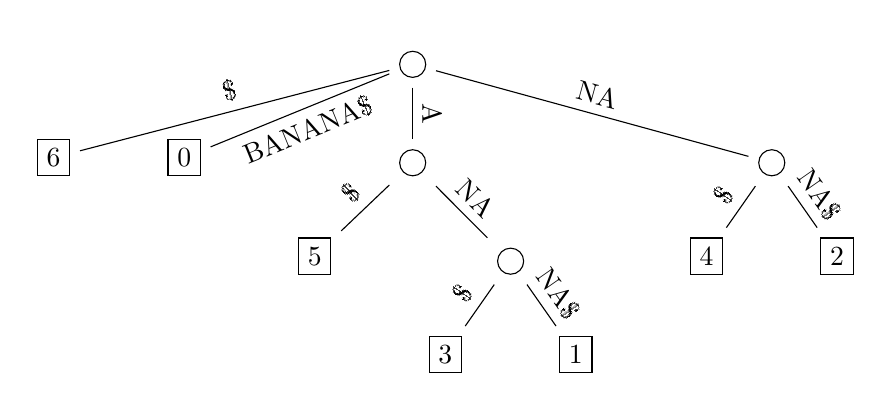
\begin{tikzpicture}[every tree node,
				level distance=1.25cm,sibling distance=1cm,
				edge from parent path={(\tikzparentnode) -- (\tikzchildnode)}]
			\Tree
			[.\addcircle{}
                \edge node[midway, above, sloped] {\$};
                [.\addsquare{6} ]
                \edge node[midway, below, sloped] {BANANA\$};
                [.\addsquare{0} ]
                \edge node[midway, above, sloped] {A};
                [.\addcircle{}
                    \edge node[midway, above, sloped] {\$};
                    [.\addsquare{5} ]
                    \edge node[midway, above, sloped] {NA};
                    [.\addcircle{}
                        \edge node[midway, above, sloped] {\$};
                        [.\addsquare{3} ]
                        \edge node[midway, above, sloped] {NA\$};
                        [.\addsquare{1} ]
                    ]
                ]
                \edge node[midway, above, sloped] {NA};
                [.\addcircle{}
                    \edge node[midway, above, sloped] {\$};
                    [.\addsquare{4} ]
                    \edge node[midway, above, sloped] {NA\$};
                    [.\addsquare{2} ]
			    ]
			]
		\end{tikzpicture}
		\caption{Suffix tree for $T=\text{BANANA\$}$}
        \label{fig:suffixtree}
	\end{center}
\end{figure}

\subsubsection{Suffix arrays}

The suffix array (SA) of a string T contains a lexicographical sorting of all suffixes in
T. The suffix array does not contain the actual suffixes, but it contains integers
pointing to the index where the suffix starts in T. Conversely, the inverse suffix array
(ISA) contains integers describing which rank the suffix at a given position has. The rank
of a suffix is its lexicographical ordering in $T$. ISA is therefore the inverse array
of SA, such that if $\text{SA}[i] = n$, then $\text{ISA}[n] = i$.

\begin{definition}[Suffix array] 
    Let T be a text of length N.
    The suffix array \texttt{SA} of T is an array of length N where $\text{SA}[i] = n$ if the
    suffix at $T[n..N-1]$ is the ith lexicographically smallest suffix in T.
\end{definition}

\begin{definition}[Inverse suffix array] 
    Let T be a text of length N.
    The inverse suffix array ISA of T is an array of length N where $ISA[i] = n$ if the
    suffix at $T[i..N-1]$ is the nth smallest suffix in T lexicographically.
\end{definition}

The Longest-common prefix (LCP) array describes how many common characters there are in a
prefix between two suffixes which are next to each other in the suffix array. Since the
suffix array represents suffixes in a sorted order, the prefix length between adjacent
suffixes in SA will be the longest possible common prefix for each suffix. These are the
values in the LCP array.

\begin{definition}[LCP array]
    Let T be a text of length N and SA be the suffix array of T.
    The LCP array of T is an array of length N where $\text{LCP[i] = n}$ if the suffix
    $\text{T[SA[i]..N]}$ and $\text{T[SA[i-1]..N]}$ has a maximal common prefix of length
    $\text{n}$. $\text{LCP[0]}$ is undefined or {0}.
\end{definition}

For example, in table \ref{table:BANANA}, the LCP value at position 3 contains the number
of characters in the longest-common prefix of suffixes starting at position 1 (ANANA\$)
and position 3 (ANA\$). These suffixes have 3 common characters in their prefix, therefore
the LCP value at position 3 is 3.

\begin{table}
	\begin{center}
        \subfloat[Suffixes]{
		\begin{tabular}{c | l }
			Index & Suffix   \\
			\hline
			0     & BANANA\$ \\
			1     & ANANA\$  \\
			2     & NANA\$   \\
			3     & ANA\$    \\
			4     & NA\$     \\
			5     & A\$      \\
			6     & \$       \\
    \end{tabular}}
		\hspace{1cm}
        \subfloat[Sorted suffixes]{\begin{tabular}{c | l}
			Index & Suffix   \\
			\hline
			6     & \$       \\
			5     & A\$      \\
			3     & ANA\$    \\
			1     & ANANA\$  \\
			0     & BANANA\$ \\
			4     & NA\$     \\
			2     & NANA\$   \\
    \end{tabular}}
		\hspace{1cm}
        \subfloat[SA, ISA and LCP]{\begin{tabular}{c | c | c | c}
                Index & SA & ISA & LCP \\
				\hline
                0     & 6  & 4   & 0\\
                1     & 5  & 3   & 0\\
                2     & 3  & 6   & 1\\
                3     & 1  & 2   & 3\\
                4     & 0  & 5   & 0\\
                5     & 4  & 1   & 0\\
                6     & 2  & 0   & 2\\
        \end{tabular}}
        \caption{$T=\text{BANANA\$}$}
        \label{table:BANANA}
	\end{center}
\end{table}


Suffix arrays can be constructed in linear time in terms of the length of T. Many suffix
array construction algorithms (SACA) have been discovered in the last
decade~\cite{SuffixArrayConstruction}, many of which run in linear-time. An algorithm which
has been shown to be very efficient in practice is Nong and Chan's algorithm based on
recursive suffix sorting of smaller strings~\cite{LinearTimeSuffixArraySAIS}. 

The enhanced (extended) suffix array is the suffix array and the additional LCP array,
which has been shown to be as powerful as a suffix tree, in terms of what can be computed
with it with the same time complexity, but uses a smaller amount of
memory~\cite{ReplaceSuffixTreeWithEnchancedSuffixArray}.

 \subsubsection{Dynamic bitsets}

A bitset is an array of bits, each bit representing either the value true or false. A bit
with the value of 1 is usually referred to as a set bit, and a value of 0 is referred to
as an unset or cleared bit. Bitsets have at least operations for setting the value at a
position, and looking up the value at a position. Bitsets are useful for many problems,
especially as a ``succinct data structure''. A succinct data structure is a data structure
which attempts to use an amount of memory close to the theoretic lower bound, while still
allowing effective queries on it. For example for a string of length $n$, we could store
up to $O(n \log_{}\sigma)$ bits before the bit vector exceeds the size of the string
itself, where $\sigma$ is the size of the string's alphabet.

The most well known query to do on bitsets is the rank/select queries.

\begin{definition}[Rank query on bitset]

    A rank query $rank_1(i)$ on a bitset B, computes the number of set bits
    up to, but not including position $i$. Conversely, $rank_0(B)$ returns the number of
    unset bits up to $i$.

\end{definition}
\begin{definition}[Select query on bitset]
    
    A select query $select_1(i)$ on a bitset B, computes the position of the ith
    set bit in B. Conversely, $select_0(i)$ returns the position of the ith unset bit in
    B.

\end{definition}

Jacobson's rank can calculate rank and select on static bitsets in $O(1)$ time by
pre-calculating all answers in a space efficient table~\cite{JacobsonsRank}.

\begin{definition}[Dynamic bitset]

    A dynamic bitset is a bitset which in addition to other operations allow inserting and
    deleting bits (indel operations).

    An insert operation $insert(i, v)$ on a bitset B inserts the value v at position i in
    B, pushing all values at position $\geq i$ one position up.

    A delete operation $delete(i)$ on a bitset B removes the value at position i in B, pushing all
    values at position $> i$ one position down.

\end{definition}

The standard implementation of a dynamic bitset would implement the whole bitset as a
single array of bytes $B$, which allows for accessing values in $O(1)$ time, but inserting
and deleting takes $O(n)$ time, where $n$ is the number of bits in $B$.

One way to speed up the indel operations would be to represent the bitset as a balanced
tree containing multiple smaller bitsets. To represent a bitset of $n$ bits, we can divide
the bits into smaller bitsets, such that $O(\frac{n}{\log(n)})$ bitsets each contains
$O(log(n))$ bits. Since the bitsets are now of size $O(log(n))$, inserting and deleting
takes only $O(log(n))$ time. The bitsets reside at the leaves of our balanced tree, and
internal nodes contain only two integers, storing the number of bits in the left subtree
($N$), and the number of set bits in the left subtree ($S$). To access, insert or delete
on index $i$, the tree is traversed to find the correct bitset where the ith bit is
located, where the operation is done at that position. Finding the correct bitset and
position is done by utilizing $N$ and $S$ in each node which is traversed. All operations
now run in $O(\log(n))$ time, since traversing the tree to the correct bitset takes
$O(\log(\frac{n}{\log(n)}))$ and performing the operation takes $O(\log(n))$ time. Keeping
the bitset balanced is done by splitting a leaf-node bitset to two nodes when the
leaf-node bitset has reached a certain size (such as $2 \times \log(n)$) and rebalancing
the tree after the split. Similarly, when considering deletions, two leaf-node bitsets can
be merged to their parent node when their combined number of bits has decreased to
$\log(n)$.


Figure \ref{fig:DynamicBitset} shows how a dynamic bitset tree is structured, and Algorithm
\ref{alg:dynbitaccess} shows how to access a value in the tree. Traversing the
tree to calculate rank and select queries can be done similarly by summing set
bits in left-subtrees (rank) or selecting which subtree to descend based on the number of
set bits (select).

\begin{figure}[t]
	\begin{center}
		\begin{tikzpicture}[every tree node,
				level distance=2cm,sibling distance=2cm,
				edge from parent path={(\tikzparentnode) -- (\tikzchildnode)}]
			\Tree
            [.\node[left, circle, draw, align=left, label={[align=left] above: $N = 8$\\$S = 3$}]{};
                \edge node[midway, above, sloped] {};
                [.\node[left, circle, draw, align=left, label={[align=left] above left:$N = 4$\\$S = 2$}]{};
                    \edge node[midway, above, sloped] {};
                    [.\addsquare{0101} ]
                    \edge node[midway, above, sloped] {};
                    [.\addsquare{0001} ]
                ]
                \edge node[midway, above, sloped] {};
                [.\node[left, circle, draw, align=right, label={[align=right] above right:$N = 4$\\$S = 1$}]{};
                    \edge node[midway, above, sloped] {};
                    [.\addsquare{0100} ]
                    \edge node[midway, above, sloped] {};
                    [.\addsquare{0000} ]
                ]
            ]
		\end{tikzpicture}
		\caption{Dynamic bitset}
        \label{fig:DynamicBitset}
	\end{center}
\end{figure}

\begin{algorithm}[htp]
  \SetAlgoLined\DontPrintSemicolon
    \algo{\access{node, i}}{
        \If{{\isLeaf{node}}}{
            \Return $\ArrayAccess{\Access{\Var{node}}{\Var{bitset}}}{\Var{i}}$
        }

        \If{$\Access{\Var{node}}{\Var{N}} \leq \Var{i}$}{
            \Return \access{$\Access{\Var{node}}{\Var{left}}, \Var{i}$}
        }

        \Return \access{$\Access{\Var{node}}{\Var{right}}, \Var{i} - \Access{\Var{node}}{\Var{N}}$}
    }

  \vspace{0.5cm}
  \caption{Accessing a value in a dynamic bitset}
  \label{alg:dynbitaccess}
\end{algorithm}

\subsubsection{Wavelet tree and wavelet matrix}

We can extend the notion of rank and select queries to strings as well. 

\begin{definition}[Rank query on string]

    A rank query $rank_c(i)$ on a string $S$ computes the number of occurrences of $c$
    in $S$ up to, but not including position $i$.

\end{definition}
\begin{definition}[Select query on string]

    A select query $select_a(i)$ on a string $S$, computes the position of the ith
    occurrence of $a$ in $S$. 

\end{definition}

The classic data structure to efficiently compute $rank$ and $select$ queries on strings
is the \textbf{wavelet tree}~\cite{WaveletTree}. The data structure is a binary tree where every
node consists of a bitset, and each level of the tree consists of the bits of a single
position in each character of the string. Each bitset in the wavelet tree can for example
be implemented as a dynamic bitset to allow indel operations on a wavelet tree.

\begin{figure}[t]
	\begin{center}
		\begin{tikzpicture}[every tree node,
				level distance=2cm,sibling distance=1.25cm,
				edge from parent path={(\tikzparentnode) -- (\tikzchildnode)}]
			\Tree
            [.\node[draw,
                align=center]{\tabbedCenterstack{a b b b e f c a g d d\\0 0 0 0 1 1 0 0 1 0 0}};
                \edge node[midway, above, sloped] {};
                [.\node[draw, align=center]{\tabbedCenterstack{a b b b c a d d\\0 0 0 0 1 0 1 1}};
                    \edge node[midway, above, sloped] {};
                    [.\node[draw, align=center]{\tabbedCenterstack{a b b b a\\0 1 1 1 0}};
                        \edge node[midway, above, sloped] {};
                        [.\addsquare{a} ]
                        \edge node[midway, above, sloped] {};
                        [.\addsquare{b} ]
                    ]
                    \edge node[midway, above, sloped] {};
                    [.\node[draw, align=center]{\tabbedCenterstack{c d d\\0 1 1}};
                        \edge node[midway, above, sloped] {};
                        [.\addsquare{c} ]
                        \edge node[midway, above, sloped] {};
                        [.\addsquare{d} ]
                    ]
                ]
                \edge node[midway, above, sloped] {};
                [.\node[draw, align=center]{\tabbedCenterstack{e f g\\0 0 1}};
                    \edge node[midway, above, sloped] {};
                    [.\node[draw, align=center]{\tabbedCenterstack{e f\\0 1}};
                        \edge node[midway, above, sloped] {};
                        [.\addsquare{e} ]
                        \edge node[midway, above, sloped] {};
                        [.\addsquare{f} ]
                    ]
                    \edge node[midway, above, sloped] {};
                    [.\node[draw, align=center]{\tabbedCenterstack{g\\0}};
                        \edge node[midway, above, sloped] {};
                        [.\addsquare{g} ]
                        \edge node[midway, above, sloped] {};
                        [.\addsquare{h} ]
                    ]
                ]
            ]
		\end{tikzpicture}
		\caption{Wavelet tree for S = abbbefcagdd}
        \label{fig:wavelettree}
	\end{center}
\end{figure}


\begin{table}[t!]
	\begin{center}
		\begin{tabular}{c}
            \begin{tabular}{c c c c c c c c c c c c}
                a & b & b & b & e & f & c & a & g & d & d \\
                \hline
            \end{tabular} \\
            \begin{tabular}{c c c c c c c c c c c c}
                0 & 0 & 0 & 0 & 1 & 1 & 0 & 0 & 1 & 0 & 0
            \end{tabular} \\
            \begin{tabular}{c c c c c c c c|c c c}
                0 & 1 & 1 & 1 & 1 & 0 & 1 & 1 & 0 & 1 & 1
            \end{tabular} \\
            \begin{tabular}{c c c c c|c c c|c c|c}
                0 & 1 & 1 & 1 & 0 & 0 & 1 & 1 & 0 & 1 & 0
            \end{tabular} \\
		\end{tabular}
		\caption{Levelwise wavelet tree}
		\label{table:levelwisewavelettree}
	\end{center}
\end{table}




Figure \ref{fig:wavelettree} shows the wavelet tree for the string \verb|abbbefcagdd|. The
wavelet tree can perform $access$, $rank$ and $select$ queries by traversing the tree from
root to leaf. 

$access(i)$ gives the bitstring of the character at a position $i$ by first accessing
position $i$ in the root bitset, if the bit is a $0$, we traverse to the left, if it is a
$1$ we traverse to the right. Before traversing to a child, we compute $rank_0(i)$ or
$rank_1(i)$, depending on what bit is at position $i$, the resulting rank is the next
position to consider in the subtree. This is done recursively until a leaf-node is found,
and the bits which were examined at each node is the bitstring of the character at
position $i$.

$rank_c(i)$ traverses the tree similarly to $access(i)$, but we use the bits of $c$ to
guide us to the correct subtree. When a leaf-node is reached, the value of $i$ is
returned, since when a leaf is reached, $i$ will be pointing to the correct rank in the
fictitious bitset of only $a$ characters

The wavelet tree can be traversed in $O(\log \sigma)$ time where $\sigma$ is the size of
the alphabet. However, the $access$, $rank$ and $select$ operations also depend on how
fast the bitsets can perform $access$, $rank$ and $select$ operations. If the bitsets are
implemented using for example Jacobson's rank~\cite{JacobsonsRank}, the bitsets have a
$O(1)$ $access$, $rank$ and $select$ time, but if we require dynamic bitsets for indel
operations, the time complexity drops to $O(\log n \log \sigma)$ because a bitset
operation which takes $O(\log n)$ time is required in each level of the tree.

The wavelet tree can also be implemented without pointers, known as a levelwise or
pointerless wavelet tree\cite{LevelwiseWaveletTree}. Table \ref{table:levelwisewavelettree}
shows the levelwise wavelet tree, which can be traversed level by level, but determining
which interval of the bitset the node you are in occupies requires two calls to $rank$.
The details of the levelwise wavelet trees are out of scope for this thesis, but leads us
into the next wavelet data structure.

The \textbf{wavelet matrix} is a relatively recent improvement on the wavelet tree, which
has been shown to be more efficient for $access$, $rank$ and $select$ queries, as well as
less memory intensive for larger alphabets~\cite{WaveletMatrix}. As the name suggests, the
wavelet matrix is a matrix of bitsets, instead of a tree of bitsets. Similarly to the
levelwise wavelet tree, for a string $S$ of size $n$, each level of the matrix consists of
a bitset of size $n$. The difference between a levelwise wavelet tree and a wavelet matrix
is that the assumption that the "children" of an interval $[x, y]$ needs to occupy exactly
$[x, y]$ is no longer true. We can instead simply put all $0$ bits to the left in the next
level, and all $1$ bits to the right. For each level we store an integer $z_l$, which
holds the number of zero bits in level $l$. 

For $access$ operations, we traverse each level similarly to a levelwise wavelet tree, but
instead of traversing a smaller and smaller interval in each level, we simply look at the
current bit at position $i$, if it is a zero, the bit to examine in the next level is
$rank_0(i)$, if the bit is a $1$, the bit to examine in the next level is $z_l +
rank_1(i)$. $rank_c(i)$ operation is carried out similarly, but we also keep track of a
preceding position to the final $i$, which we subtract from $i$, to count only the number
of proceeding number of $a$ characters. Table \ref{table:waveletmatrix} shows an example
wavelet matrix, and algorithm \ref{alg:waveletmatrixaccess} and
\ref{alg:waveletmatrixrank} shows how $access$ and $rank$ operations can be carried out
for a wavelet matrix.

\begin{table}[t]
	\begin{center}
		\begin{tabular}{c}
            \begin{tabular}{c c c c c c c c c c c c}
                a & b & b & b & e & f & c & a & g & d & d \\
                \hline
                0 & 0 & 0 & 0 & 1 & 1 & 0 & 0 & 1 & 0 & 0 \\
                0 & 0 & 0 & 0 & 1 & 0 & 1 & 1 & 0 & 0 & 1 \\
                0 & 1 & 1 & 1 & 0 & 0 & 1 & 0 & 1 & 1 & 0
            \end{tabular} \\
		\end{tabular}
		\caption{Wavelet matrix for S = abbbefcagdd}
		\label{table:waveletmatrix}
	\end{center}
\end{table}


\begin{figure}
\begin{minipage}{0.46\textwidth}
    \begin{algorithm}[H]
        \SetAlgoLined\DontPrintSemicolon
        \algo{\access{WM, i}}{
            $\Var{bits} \gets \textrm{empty\ list}$ \;
            $\Var{l} \gets 0$ \;
            \While{$\Var{l} < \Len{$\Var{WM}$}$}{
                \Add{$\Var{bits}, \access{$\ArrayAccess{\Var{WM}}{\Var{l}}, \Var{i}$}$} \;
                \uIf{$\access{$\ArrayAccess{\Var{WM}}{\Var{l}}, \Var{i}$} = 1$}{
                    $\Var{i} \gets z_l + \RankOne{$\ArrayAccess{\Var{WM}}{\Var{l}}, \Var{i}$}$ \;
                }
                \Else{
                    $\Var{i} \gets \RankZero{$\ArrayAccess{\Var{WM}}{\Var{l}}, \Var{i}$}$ \;
                }
                $\Var{l} \gets \Var{l} + 1$
            }
            \Return $\Var{bits}$ \;
        }
        \caption{Wavelet matrix access}
        \label{alg:waveletmatrixaccess}
    \end{algorithm}
\end{minipage}
\begin{minipage}{0.46\textwidth}
    \begin{algorithm}[H]
        \SetAlgoLined\DontPrintSemicolon
        \algo{\RankC{WM, i}}{
            $\Var{l} \gets 0$ \;
            $\Var{p} \gets 0$ \;
            \While{$\Var{l} < \Len{$\Var{WM}$}$}{
                \uIf{$\access{$\ArrayAccess{\Var{WM}}{\Var{l}}, \Var{i}$} = 1$}{
                    $\Var{i} \gets z_l + \RankOne{$\ArrayAccess{\Var{WM}}{\Var{l}}, \Var{i}$}$ \;
                    $\Var{p} \gets z_l + \RankOne{$\ArrayAccess{\Var{WM}}{\Var{l}}, \Var{p}$}$ \;
                }
                \Else{
                    $\Var{i} \gets \RankZero{$\ArrayAccess{\Var{WM}}{\Var{l}}, \Var{i}$}$ \;
                    $\Var{p} \gets \RankZero{$\ArrayAccess{\Var{WM}}{\Var{l}}, \Var{p}$}$ \;
                }
                $\Var{l} \gets \Var{l} + 1$
            }
            \Return $\Var{i} - \Var{p}$ \;
        }
        \caption{Wavelet matrix rank}
        \label{alg:waveletmatrixrank}
    \end{algorithm}
\end{minipage}
\end{figure}

The wavelet matrix is constructed level by level. In level $i$, the bit at position $i$ in
each character is inserted. Before constructing the next level, each character is sorted
by the current bit, so that all the characters with $0$ bits at position $i$ occupies the
left side of level $i + 1$, and vice versa for $1$ bits.

\subsubsection{Burrows-Wheeler transform}

\begin{table}[t]
	\begin{center}
        \subfloat[Cyclic shifts]{
		\begin{tabular}{c | l }
			Index & Cyclic-shift   \\
			\hline
			0     & BANANA\$ \\
			1     & ANANA\$B \\
			2     & NANA\$BA \\
			3     & ANA\$BAN \\
			4     & NA\$BANA \\
			5     & A\$BANAN \\
			6     & \$BANANA \\
    \end{tabular}}
		\hspace{0.5cm}
        \subfloat[Sorted cyclic shifts and BWT]{\begin{tabular}{c | l}
			Index & Cyclic-shift   \\
			\hline
            6     & \$BANAN\textbf{A} \\
            5     & A\$BANA\textbf{N} \\
			3     & ANA\$BA\textbf{N} \\
			1     & ANANA\$\textbf{B} \\
			0     & BANANA\textbf{\$} \\
			4     & NA\$BAN\textbf{A} \\
			2     & NANA\$B\textbf{A} \\
    \end{tabular}}
		\hspace{0.5cm}
        \subfloat[LF function]{\begin{tabular}{c | l}
			L & F   \\
			\hline
            0     & $Rank_A(0) + C[A] = 0 + 1 = 1$\\
            1     & $Rank_N(1) + C[N] = 0 + 5 = 5$ \\
			2     & $Rank_N(2) + C[N] = 1 + 5 = 6$ \\
			3     & $Rank_B(3) + C[B] = 0 + 4 = 4$ \\
            4     & $Rank_{\$}(4) + C[\$] = 0 + 0 = 0$ \\
			5     & $Rank_A(5) + C[A] = 1 + 1 = 2$ \\
			6     & $Rank_A(6) + C[A] = 2 + 1 = 3$ \\
    \end{tabular}}
    \caption{S = BANANA\$, BWT = ANNB\$AA}
    \label{table:bwt}
	\end{center}
\end{table}

The Burrows-Wheeler transform (BWT) is a transform on strings, often performed on strings
to improve compression~\cite{BWT}. The transform is computed by sorting all
``cyclic-shifts'' of the string lexicographically and extracting a new string from the
last column of the cyclic-shift'' matrix. \$ is added to the string as a unique
terminating character, this makes some of the algorithms on the BWT simpler. \$ is always
the smallest character lexicographically. Table \ref{table:bwt} shows the BWT for the
string S = BANANA\$.

\begin{definition}{Cyclic-shift}

    The cyclic-shift of order $i$ for a string $S$ is the cyclic-shift of $S$ such that
    all characters in $S$ are rotated $i$ characters to the left. The cyclic-shift of
    order $i$ is denoted $CS_i$

\end{definition}

\begin{definition}{Burrows-Wheeler transform}

    The Burrows-Wheeler transform of a string $S$ is a transformation on $S$ where the
    cyclic-shifts of $S$ are sorted, and the final character in each shift is concatenated.

\end{definition}

There is a direct correlation between the suffix array of S and the BWT of S. Table
\ref{table:bwt} also shows that the indices of the sorted cyclic-shifts correspond to
exactly the SA of S. This coincides because when sorting cyclic-shifts, everything that
occurs after the \$ of the cyclic-shift will not affect its lexicographical ordering. This
is because no cyclic-shift will have a \$ in the same position, so comparing two cyclic
shifts lexicographically will always terminate whenever a \$ is found. This means that the
ordering of cyclic shifts is essentially the same as sorting all suffixes of S. Algorithm
\ref{alg:bwt} shows how the BWT of S can be calculated directly from the SA of S in linear
time. Since this is a one to one correlation between the SA and BWT, dynamic updates to a BWT
would correspond to similar dynamic updates in the SA (and ISA). This will be useful in
the following implementation chapter for the dynamic code clone detection algorithm.

\begin{algorithm}[htp]
  \SetAlgoLined\DontPrintSemicolon
    \algo{\ComputeBWT{S, SA}}{
        $\Var{n} \gets \Access{S}{len}$

        $BWT \gets \mathrm{string\ of\ length\ } n$

        \For{$i \From 0 \To \Var{n}$}{

            $\Var{pos} \gets (\SA{\Var{i}} - 1)\ \%\ n$

            $\BWT{i} = \ArrayAccess{\Var{S}}{pos}$
        }

        \Return BWT
    }

  \vspace{0.5cm}
  \caption{Calculating the BWT of a string T from its suffix array}
  \label{alg:bwt}
\end{algorithm}


An essential property of the BWT is that the transformation is reversible. By examining
the BWT of a string T, we see that the BWT is a permutation of T. We will also see that
there is a correlation between the characters in the first column of the cyclic-shift
matrix and the last column (the BWT).

T can be calculated from the BWT as long as there is a unique terminating character (\$),
or the position of the final character is stored. T is computed backwards by starting at
the final character ($T[n - 1]$) and then finding the cyclic-shift where that character
occurs in the first column (the previous cyclic-shift). The character in the last column
of that cyclic-shift is $T[n - 2]$. If there are multiple of the same character, the nth
occurrence of a certain symbol in the last column will map to the nth occurrence of the
same symbol in the first column. This process is repeated until we finish the cycle,
returning to the final character in the last column. Essentially, this process consists of
traversing cyclic-shifts backwards and looking at the final character, which will give us
T, since the final character of the cyclic-shift is continually shifting one position.

We can use the fact that the first column consists of the letters of T in sorted order to
determine the previous cyclic-shift with only the last column. We can calculate the
previous cyclic-shift from only the last column by determining how many characters are
lexicographically smaller than the current character, and also the rank of the current
character at this position. The sum of these two values is the location of the previous
cyclic-shift. This function is called the Last-to-first function (LF function).
Calculating the LF function can be done efficiently by using a rank/select data structure
such as a wavelet tree~\cite{WaveletTree} or wavelet matrix~\cite{WaveletMatrix} to
calculate the rank of all the characters in the BWT, and an array $C$ which contains the
number of occurrences of each letter in the BWT.

The LF function will also be useful in the detection algorithm when dynamically updating
the suffix array.

\chapter{Implementation}


\subsection{Architecture of tool}

\begin{figure}
	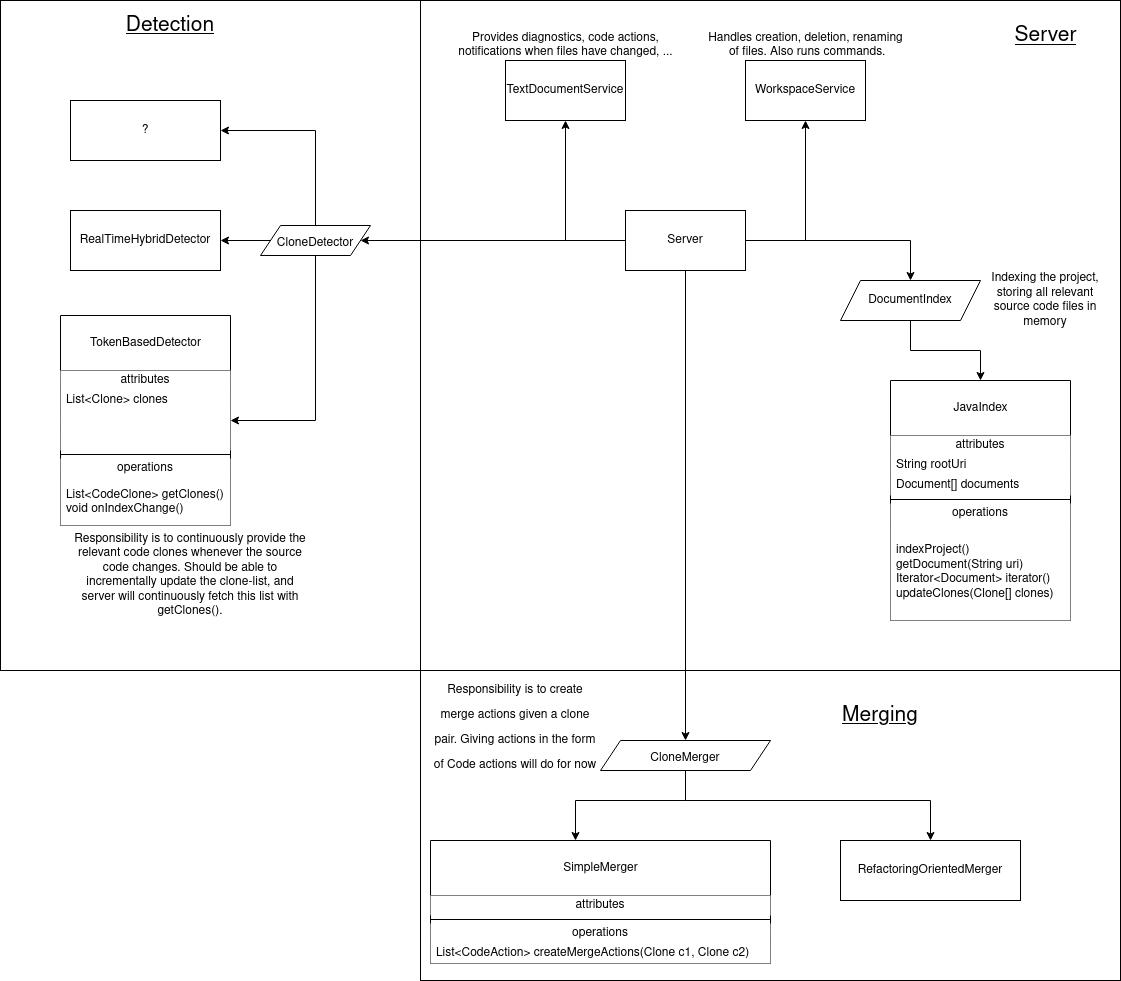
\includegraphics[width=\textwidth]{images/ToolArchitecture.png}
	\caption{Tool architecture}
	\label{fig:architecture}
\end{figure}

Figure \ref{fig:architecture} shows the architecture of the tool. The server communicates
with the IDE and delegates the work of managing clones to the detection engine and the
merge engine. The tool also stores an index of all source code files in the current project.

\chapter{Evaluation}


We will evaluate this tool based on different criteria, which combined will provide a
basis for evaluating the tool as a whole.

Since the tool is focused on efficient detection and management of code clones, real-time
performance of the tool will be a high priority in its evaluation. The tool will implement
different techniques of detecting and merging clones. These will be empirically compared
against each other. The tool will also be evaluated against existing tools empirically. We
will utilize BigCloneBench~\cite{BigCloneBench} to evaluate detection techniques, by
running our detection techniques in a standalone mode. We will distinguish between initial
detection and incremental detection when evaluating.

The tool will also be evaluated in how well it fits into the software development cycle.
Can we determine if this tool is an effective way to detect a clone early in its lifecycle
so that they can be removed before it manifests in the source code? In relation to this,
we will evaluate if LSP is a suitable tool for use in clone management and refactoring in
general. Can LSP provide all the features one would want in a modern analysis tool? What
is missing, and how could the LSP protocol be extended in order to facilitate this? We
believe that if LSP is an appropriate tool to use for clone management, LSP will also be
an appropriate tool for static analysis tools in general.


\chapter{Discussion}

\section{Performance}

\section{Clones}

\chapter{Conclusion and future work}

The results show that CCDetect incremental algorithm outperforms the other two algorithms
both in terms of time and memory on larger code bases. Our algorithm was able to handle
large edits in an IDE environment for 5.8MLOC in under 2 second,

\section{Future work}

In this section we list future work and research in order of what we consider
most interesting to do more research on, to least.

\subsection*{Type-2 and type-3 clones}

\subsection*{Optimal edit operations}

\subsection*{Refactoring of clones}

\subsection*{Compressing data structures}

\subsection*{Lazy LCP array updates}

\section{Related work}


\section{Conclusion}


\printbibliography
\end{document}
